\documentclass{article}
\usepackage[utf8]{inputenc}
\usepackage[margin=0.35in]{geometry}


\title{Computer Networks Lab 6}
\author{Shane Cincotta }
\date{May 11, 2020}

\usepackage{natbib}
\usepackage{graphicx}

\begin{document}

\maketitle
\begin{figure}[h!]
\centering
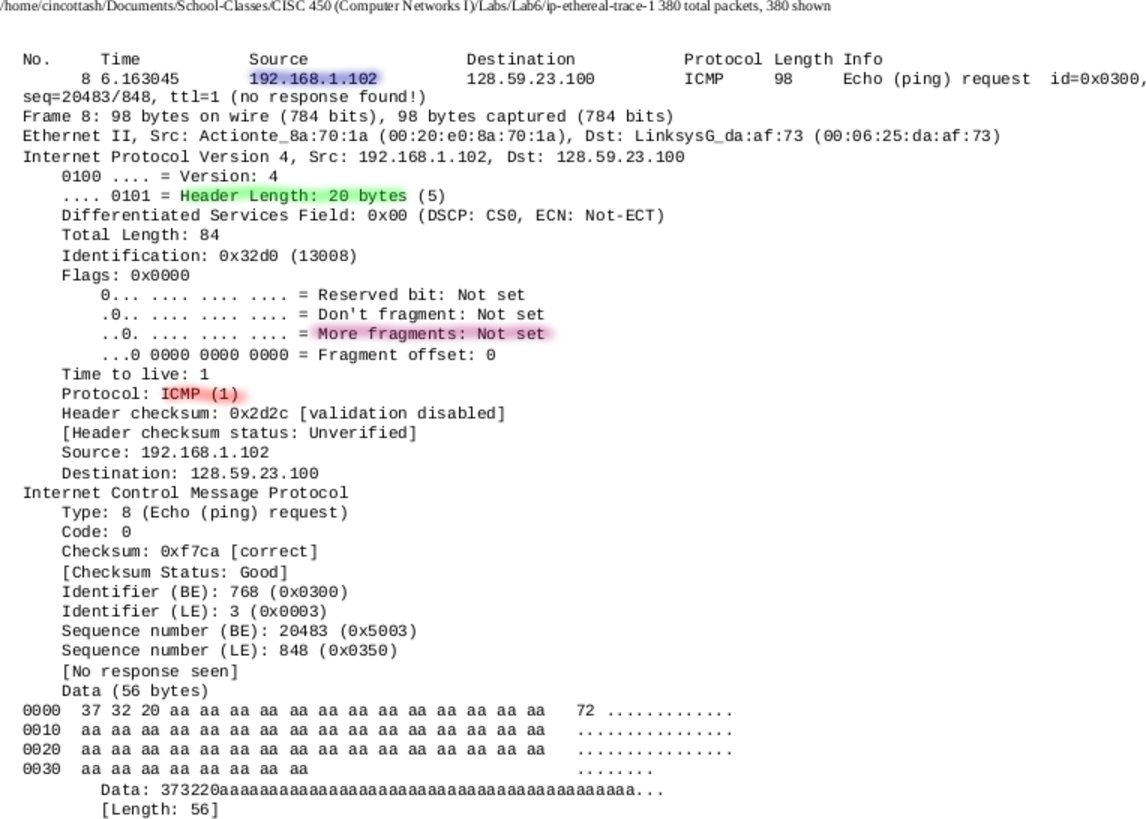
\includegraphics[scale=0.65]{Q1-4.pdf}
\caption{}
\end{figure}

\section*{What is the IP address of your computer?}
According to figure 1, the IP address of my computer is 192.168.1.102.\\

\section*{Within the IP packet header, what is the value in the upper layer protocol field?}
According to figure 1, the value in the upper layer protocol field is ICMP (1).\\

\section*{How many bytes are in the IP header? How many bytes are in the payload of the
IP datagram? Explain how you determined the number of payload bytes.}
According to figure 1, there are 20 bytes in the IP header.  There are 36 bytes in the payload.  This can be calculated by subtracting the IP header size (20) from the total data size (56).\\

\section*{Has this IP datagram been fragmented? Explain how you determined whether or
not the datagram has been fragmented}
According to figure 1, the data has not been fragmented.  This can be determined by by the value of the more fragments bit, which is set to 0.\\

\begin{figure}[h!]
\centering
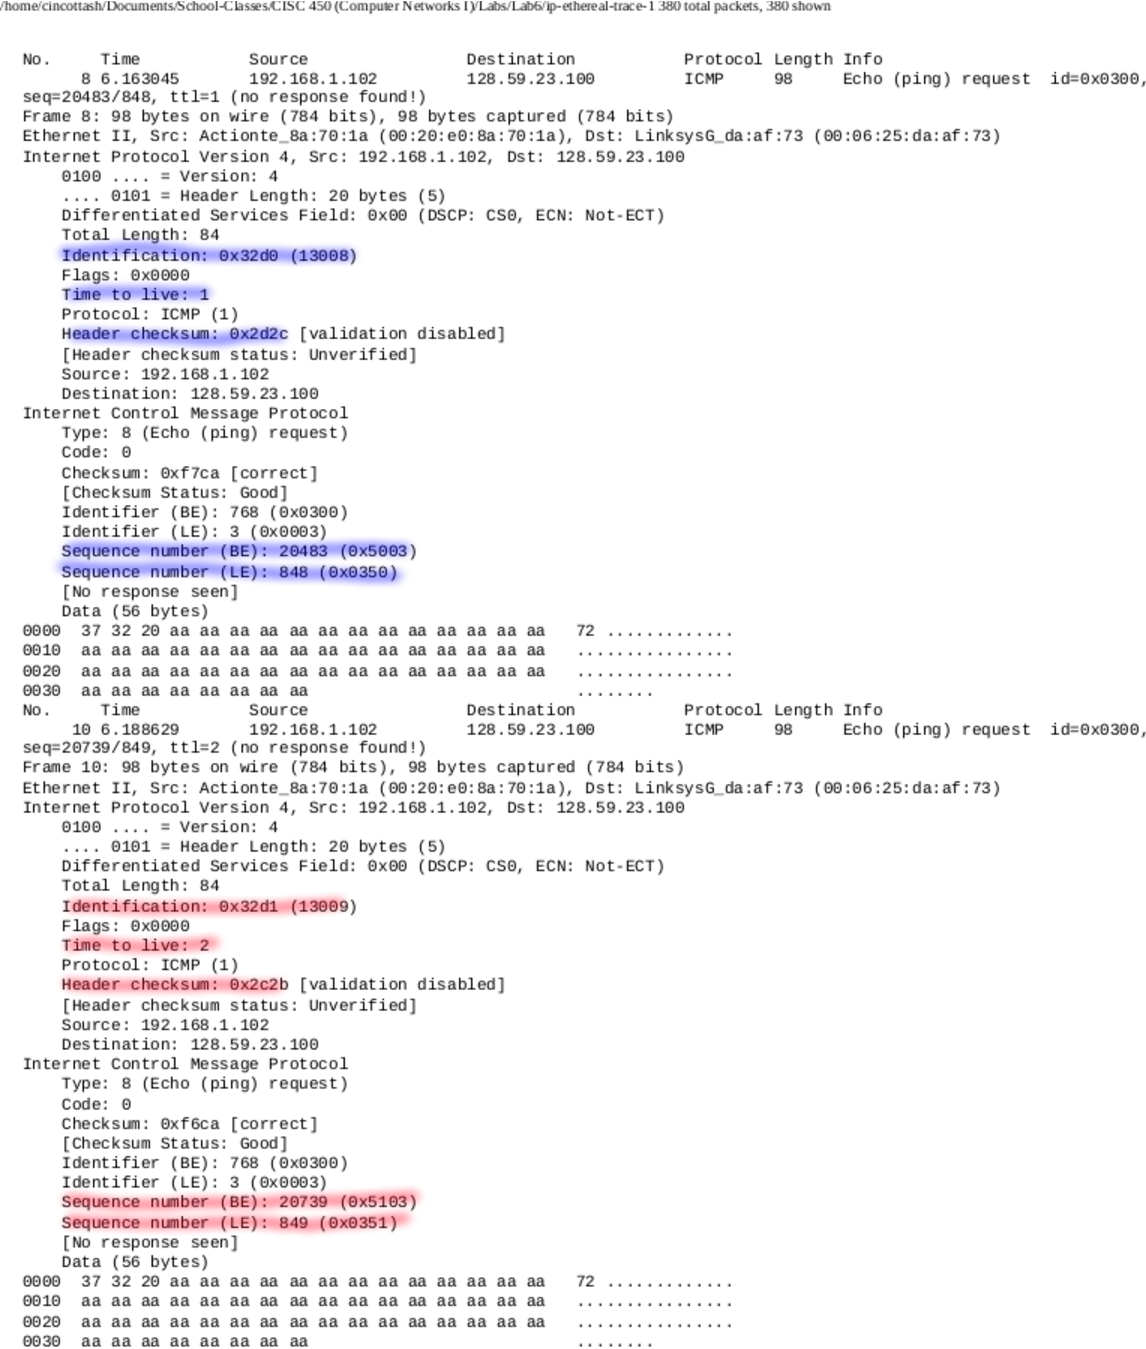
\includegraphics[scale=0.5]{Q5.pdf}
\caption{}
\end{figure}

\section*{Which fields in the IP datagram always change from one datagram to the next
within this series of ICMP messages sent by your computer?}
According to figure 2, the Identification, Time to live, Header checksum and sequence number never change.\\
\clearpage

\begin{figure}[h!]
\centering
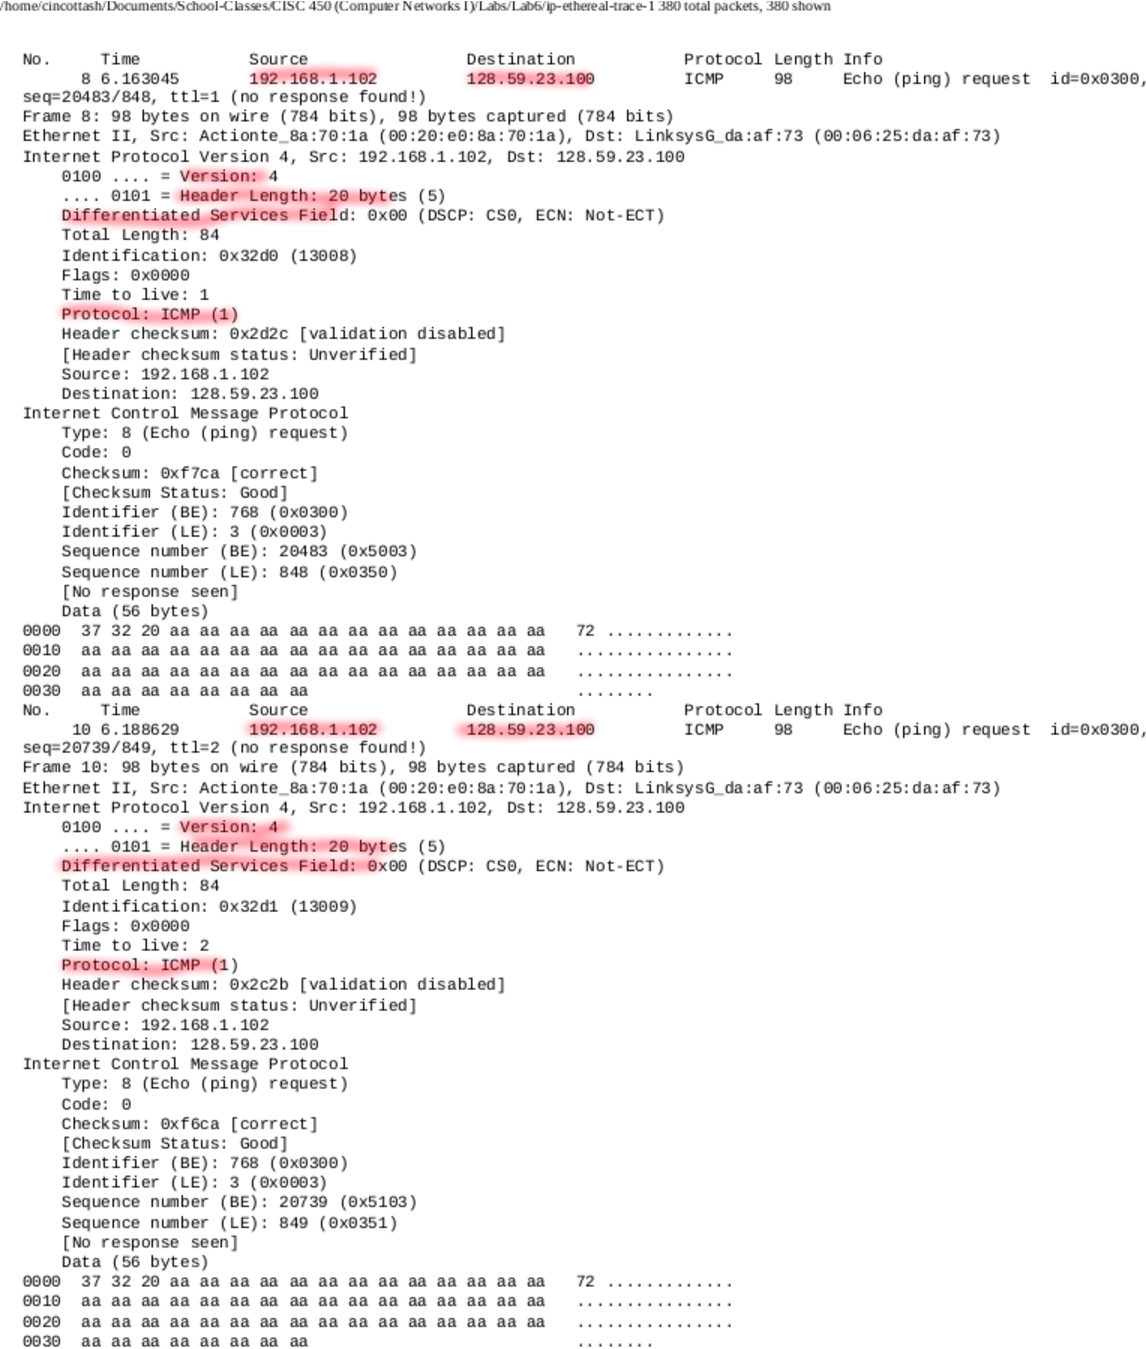
\includegraphics[scale=0.5]{Q6.pdf}
\caption{}
\end{figure}

\section*{Which fields stay constant? Which of the fields must stay constant? Which fields
must change? Why?}
According to figure 3: version, header length, source IP, destination IP differentiated services and upper layer protocol all remain constant.\\
\newline The fields that must stay constant are: version (because we are using IPv4), header length (because each packet is ICMP), source IP (because we are sending from the same source PC), destination IP (because we are sending to the same source PC), differentiated services (because each packet is ICMP thus they use the same type of service) and upper layer protocol (because each packet is ICMP).\\
\newline The fields that must change are: identification (because each packet has a different ID), time to live (because each TTL is incremented after each packet) and header checksum (because the checksum changes along with the header).\\

\clearpage

\begin{figure}[h!]
\centering
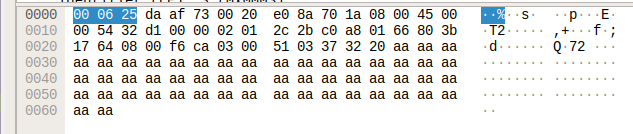
\includegraphics[scale=0.5]{Q7.png}
\caption{}
\end{figure}

\section*{Describe the pattern you see in the values in the Identification field of the IP
datagram}
According to figure 4, the pattern I observe is that the IP header Identification fields increment after each ICMP Echo.\\

\begin{figure}[h!]
\centering
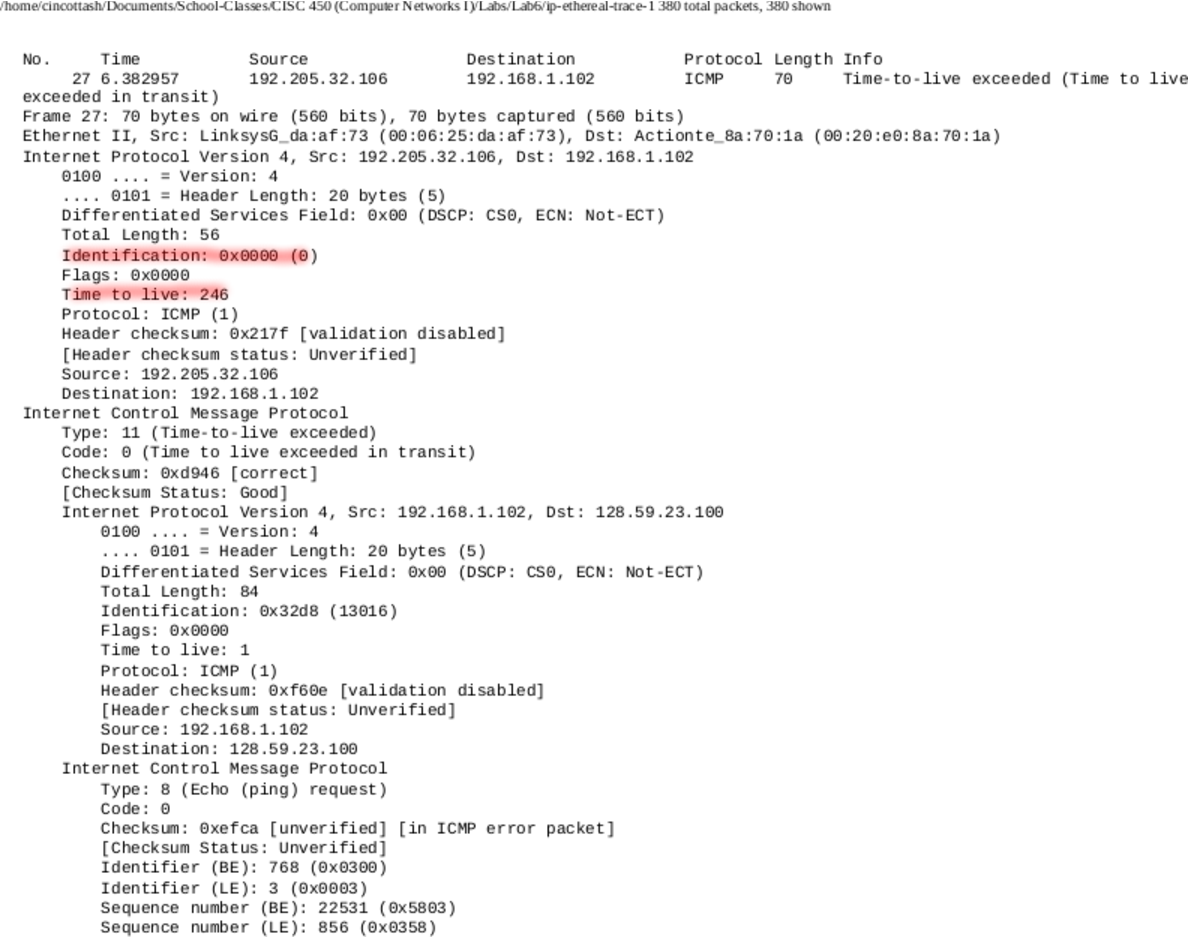
\includegraphics[scale=0.5]{Q8.pdf}
\caption{}
\end{figure}

\section*{What is the value in the Identification field and the TTL field?}
According to figure 5, the value of the indentification field is 0 and the value of the TTL field is 246.\\
\clearpage

\begin{figure}[h!]
\centering
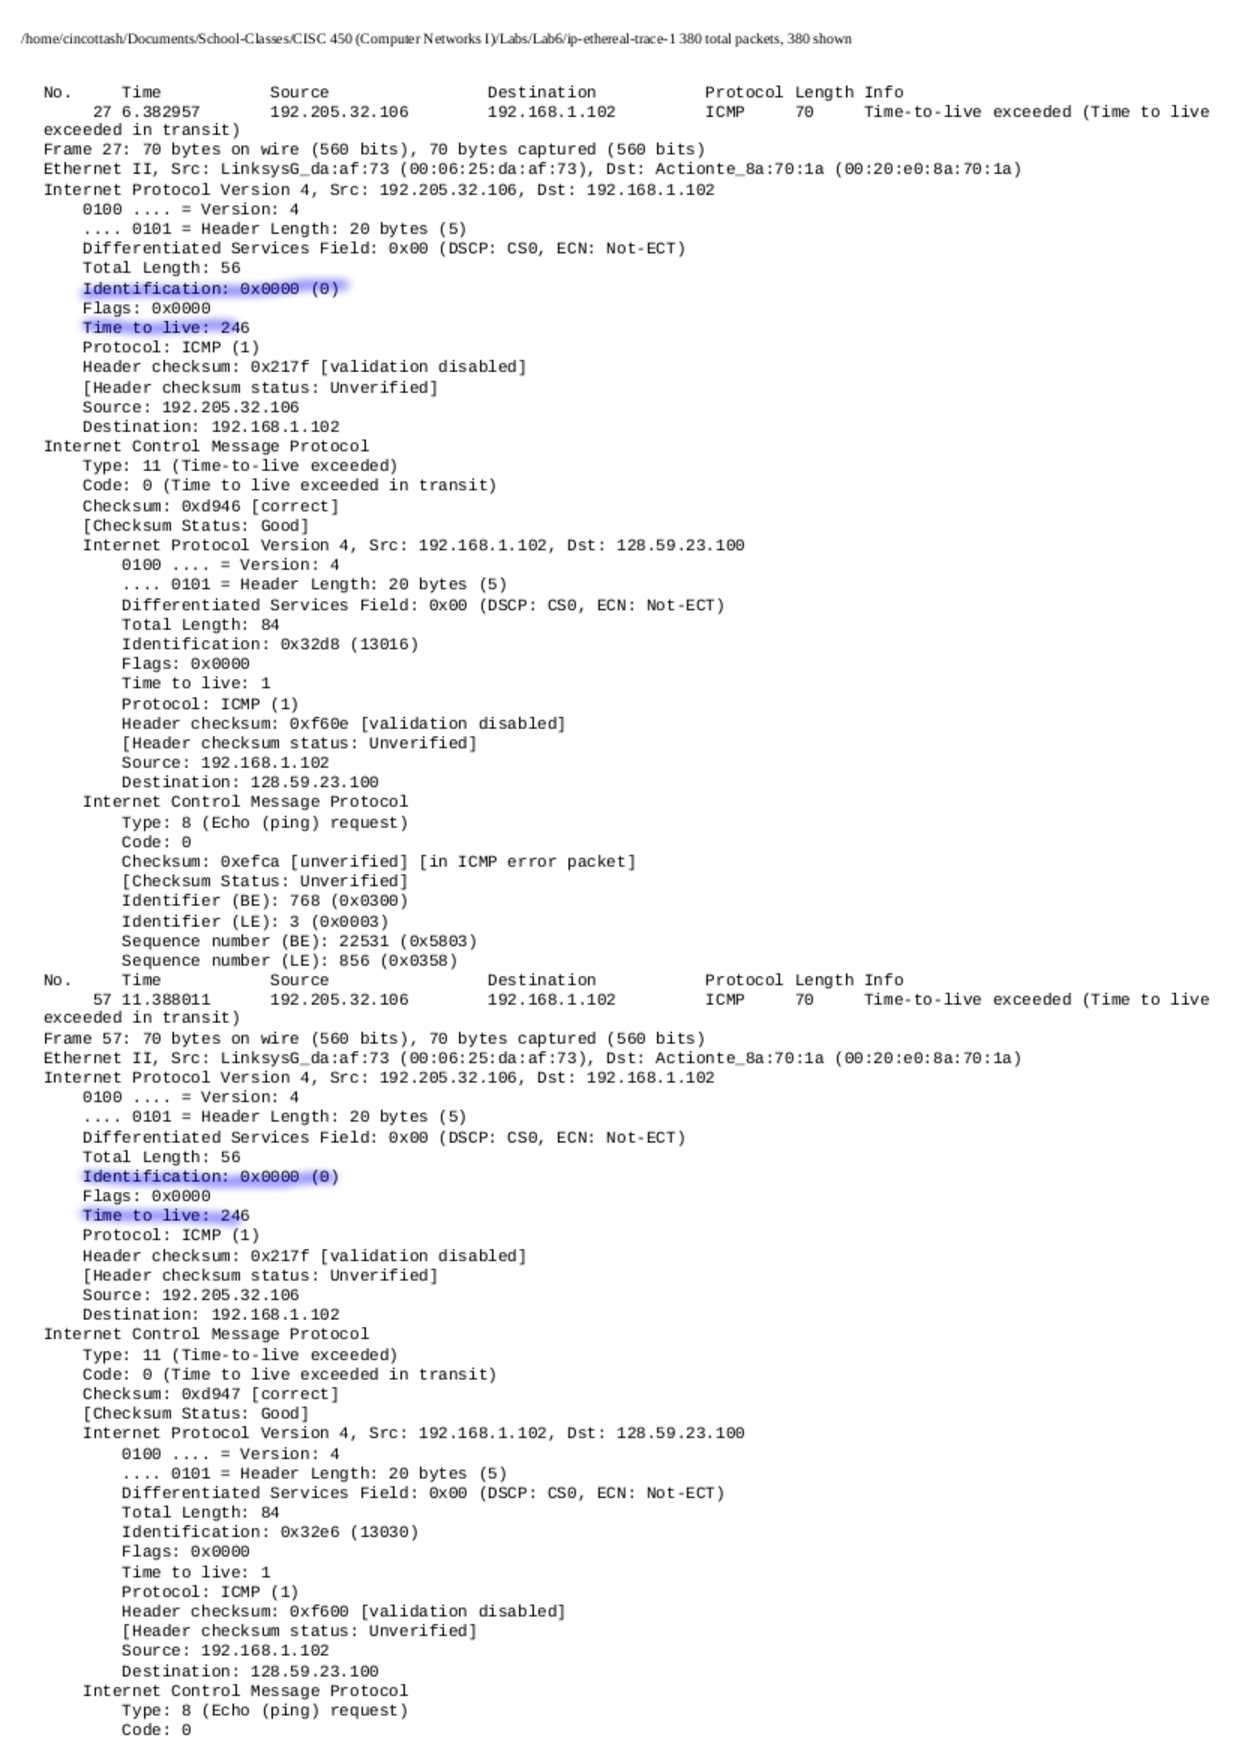
\includegraphics[scale=0.5]{Q9.pdf}
\caption{}
\end{figure}

\section*{Do these values remain unchanged for all of the ICMP TTL-exceeded replies sent
to your computer by the nearest (first hop) router? Why?}
According to figure 6, the identification field does not change.  The reason for this is when two or more IP datagrams have the same ID value, they are fragments of a larger IP datagram.\\
\newline  According to figure 6, the TTL fields remains unchanged because the TTL for the first hop router is always the same.\\
\clearpage

\begin{figure}[h!]
\centering
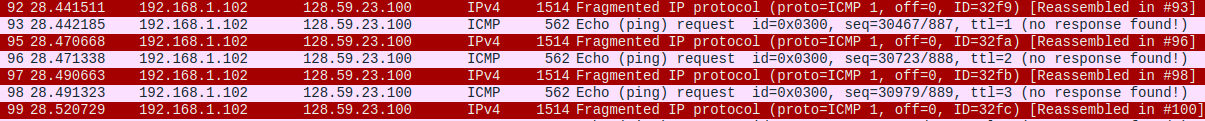
\includegraphics[scale=0.5]{Q10.png}
\caption{}
\end{figure}

\section*{Find the first ICMP Echo Request message that was sent by your computer after
you changed the Packet Size in pingplotter to be 2000. Has that message been
fragmented across more than one IP datagram?}

According to figure 7, this packet has been fragmented across more than one IP diagram.\\

\begin{figure}[h!]
\centering
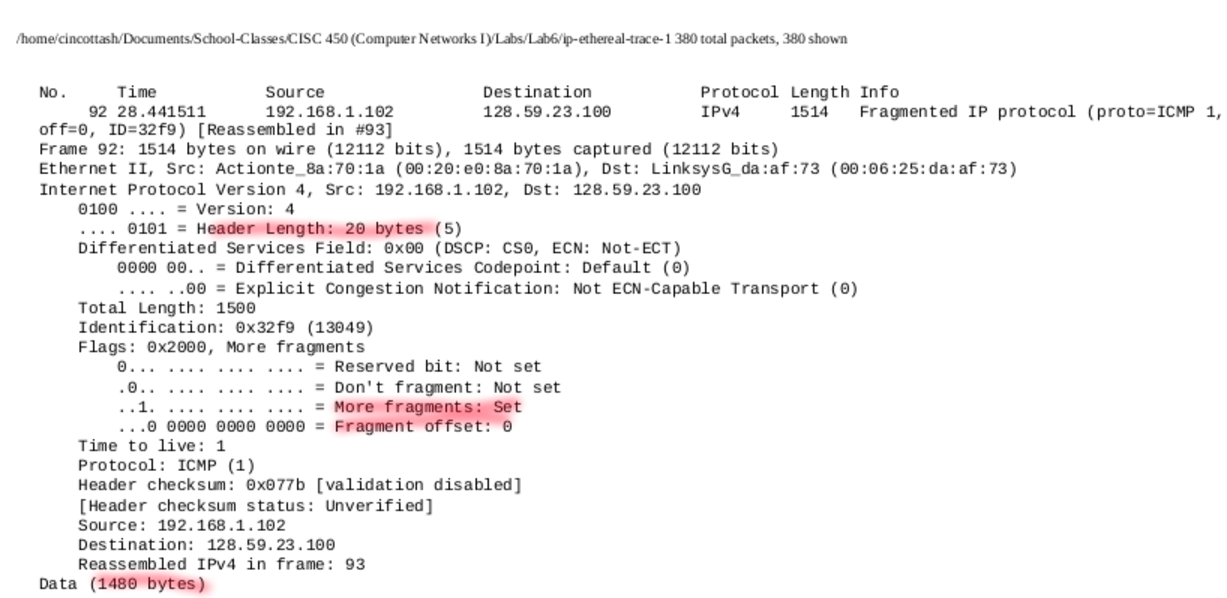
\includegraphics[scale=0.5]{Q11.pdf}
\caption{}
\end{figure}

\section*{Print out the first fragment of the fragmented IP datagram. What information in
the IP header indicates that the datagram been fragmented? What information in
the IP header indicates whether this is the first fragment versus a latter fragment?
How long is this IP datagram?}
According to figure 8, the flags bit for more fragments is set, this tells us that the datagram is fragmented.  Also, since the fragment offset is 0, we know that this is the first fragment.  This datagram has a total length of 1500 (1480 + header size).\\

\begin{figure}[h!]
\centering
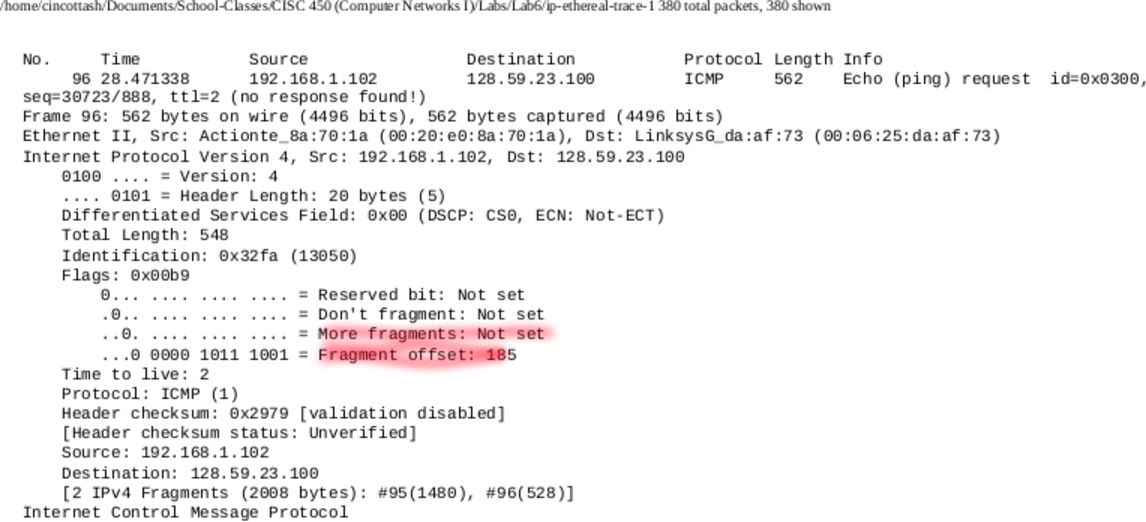
\includegraphics[scale=0.5]{Q12.pdf}
\caption{}
\end{figure}

\section*{Print out the second fragment of the fragmented IP datagram. What information in
the IP header indicates that this is not the first datagram fragment? Are the more
fragments? How can you tell?}
According to figure 9, we can tell that this is not the first fragment because the fragment offset is 185, also we know it is the last fragment because the more fragments flag is not set.\\

\begin{figure}[h!]
\centering
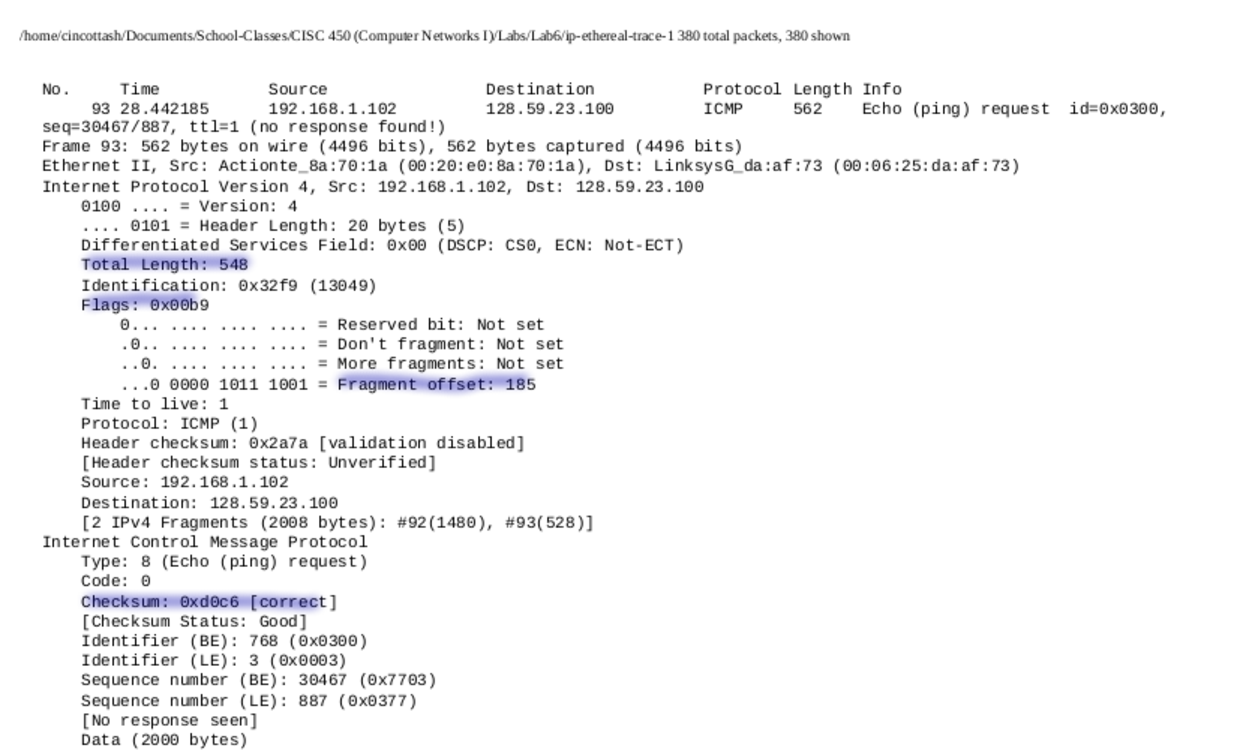
\includegraphics[scale=0.5]{Q13.pdf}
\caption{}
\end{figure}

\section*{What fields change in the IP header between the first and second fragment?}
According to figure 10, we can see that the total length, checksum, flags and dragment offset are changed.

\begin{figure}[h!]
\centering
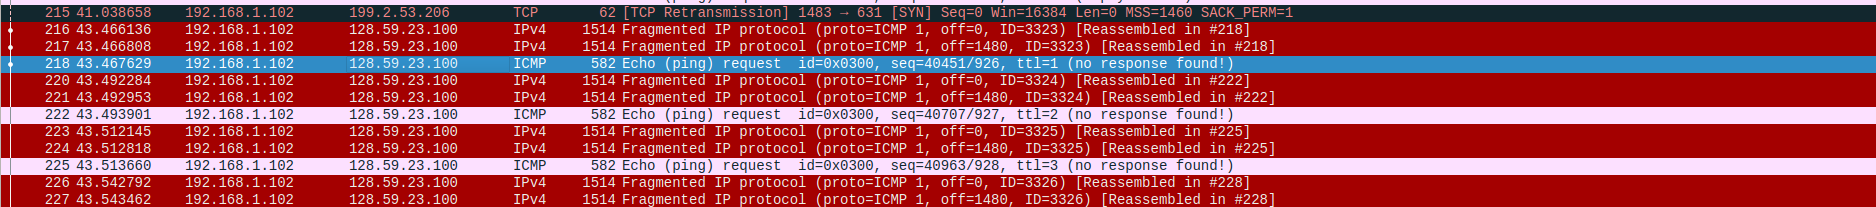
\includegraphics[scale=0.5]{Q14.png}
\caption{}
\end{figure}

\section*{How many fragments were created from the original datagram?}
According to figure 11, after switching to 3500, there are 3 packets created.\\
\clearpage

\begin{figure}[h!]
\centering
\includegraphics[scale=0.5]{Q15.pdf}
\caption{}
\end{figure}

\section*{What fields change in the IP header among the fragments?}
According to figure 12, the fragment offset and checksum change among the fragments.

\end{document}